% ------------------------------------------
% M2I SOP Template
% ------------------------------------------

% Preamble
\newcommand{\mytitle}{M2I Project Development and Implementation Plan (PDIP)}
\newcommand{\myauthors}{Project Manager Name}
\newcommand{\mydate}{\today \\ Revision 1.0}
% Revisions must be incremented based on the following.
% Each new semester triggers a major revisions number eg 2.0, 3.0, 4.0, etc
% Each revision during the semester is a minor revision number, eg 1.1, 1.2, 1.5, etc

% M2I Formal Report Template
% ------------------------------------------

\documentclass[letterpaper,11pt]{article}

% begin package imports -- {{{
\usepackage{graphicx}
\usepackage[dvipsnames,table]{xcolor}
\usepackage{tabto}
\usepackage{titling}
%\usepackage[iso,english]{isodate}
\usepackage{tabu}
\usepackage[intoc]{nomencl}
\makenomenclature
\usepackage{datetime}
\usdate
\usepackage[T1]{fontenc}
\usepackage{algorithmic,algorithm}
\usepackage{color}
\usepackage{listings,url}
\usepackage{pdfpages}
\usepackage{wallpaper}
\usepackage{titlesec}
\usepackage{enumitem}
\usepackage{changepage}
\usepackage{pdfpages}
\usepackage{lscape}
\usepackage{amsmath}
\usepackage{montserrat}

% ------------------------------------------
% ToC, AIAA-style Bibliography
\usepackage[immediate]{silence}
\WarningFilter{latex}{You have requested package}
\usepackage[tocgraduated]{assets/tocstyle}
\usetocstyle{standard}
\RequirePackage[sort&compress,numbers]{natbib}
\bibliographystyle{new-aiaa}
\WarningFilter[temp]{latex}{Command}
    \usepackage{sectsty}
\DeactivateWarningFilters[temp]
\usepackage[nottoc]{tocbibind}

% ------------------------------------------
% Figures & tables
\usepackage{float}
\usepackage[small,bf]{caption}
\usepackage{subcaption}
\usepackage{tabularx}
\usepackage{multirow}
\usepackage{placeins}
\usepackage{makecell}
\usepackage[figuresleft]{rotating}

% ------------------------------------------
% Custom layout parameters
\usepackage[margin=0.75in]{geometry}
\definecolor{MASA-Blue}{RGB}{0,39,76}
\renewcommand\thesection{\Roman{section}}
\renewcommand{\bibsection}{\section{References}}
\newcommand{\boldheader}[1]{\vspace{5mm}\textbf{#1}\textbf{:}\newline}
\sectionfont{\fontsize{19}{20}\color{MASA-Blue}\fontseries{b}\fontfamily{Montserrat-TOsF}\selectfont}
\subsectionfont{\fontsize{16}{18}\color{MASA-Blue}\fontfamily{Montserrat-TOsF}\selectfont}
\subsubsectionfont{\fontseries{sb}\fontshape{n}\color{MASA-Blue}\fontfamily{Montserrat-TOsF}\selectfont}
\titlespacing{\subsection}{0pt}{100mm}{0pt}
\setlength{\parindent}{0in}
\setlength{\parskip}{1em}

% end package imports -- }}}

% begin set section title styles -- {{{

%\titleformat{\section} {\setcounter{checklistnum}{0} \normalfont\Large\bfseries}{}{0em}{}[{\titlerule[0.8pt]}]
%\titleformat{\subsection} {\setcounter{checklistnum}{0} \normalfont\large}{}{0em}{}[{\titlerule[0.6pt]}]
% end set section title styles -- }}}

% begin checklist symbols definition -- {{{
\usepackage{enumitem,amssymb}
\newcounter{checklistnum}
\setcounter{checklistnum}{0}
\DeclareRobustCommand{\checklistnumber}{\refstepcounter{checklistnum}\thechecklistnum}
\newlist{checklist}{itemize}{6}
\setlist[checklist,1]{
label={\color{gray}\checklistnumber}\hspace{2em}$\square$,
leftmargin=0em,
itemindent=2em
}
\setlist[checklist,2]{
label={\color{gray}\checklistnumber}\hspace{4em}$\square$,
leftmargin=0em,
itemindent=4em
}
\setlist[checklist,3]{
label={\color{gray}\checklistnumber}\hspace{6em}$\square$,
leftmargin=0em,
itemindent=6em
}
\setlist[checklist,4]{
label={\color{gray}\checklistnumber}\hspace{8em}$\square$,
leftmargin=0em,
itemindent=8em
}
\setlist[checklist,5]{
label={\color{gray}\checklistnumber}\hspace{10em}$\square$,
leftmargin=0em,
itemindent=10em
}
\setlist[checklist,6]{
label={\color{gray}\checklistnumber}\hspace{12em}$\square$,
leftmargin=0em,
itemindent=12em
}
% end checklist symbols definition -- }}}

\newcommand{\GO}{\textcolor{green}{\textbf{GO }}}
\newcommand{\NOGO}{\textcolor{red}{\textbf{NO-GO }}}

% begin personnel macro -- {{{
\newcommand{\operator}[4]{%
  \expandafter\newcommand\csname #1\endcsname{{\color{#2}\textbf{#3}}\phantom{}}
  \expandafter\newcommand\csname #1full\endcsname{{\color{#2}\textbf{#4 [#3]}}\phantom{}}
}
% end personnel macro -- }}}

% begin flag macro -- {{{
\newcommand\flag[1]{
    \hfill \makebox(0,0){\hspace{1.7in}\textcolor{#1}{\rule{0.3in}{0.5in}}}
}
% end flag macro -- }}}

\pagenumbering{gobble}


\newcommand\signature[2]{
    \begin{minipage}{5cm}
        \noindent\vspace{4.5mm}\par
        \noindent\vspace{-1mm}\rule{#1cm}{0.5pt}\par
        \noindent#2
    \end{minipage}
}

% ------------------------------------------
% Title Page
\newcommand\makeTitlePage[1]{
    \newpage
    \ClearWallPaper
    \thispagestyle{empty}
    \setlength{\parskip}{0in}
    \LLCornerWallPaper{1}{assets/Footer4.pdf}
    \vspace*{\fill}
    \begin{adjustwidth}{1.5cm}{1.5cm} 
    \begin{center}
        
\includegraphics[width=7cm]{assets/M2I Logo Clean.png}\\
        \vspace{20mm}
        \fontsize{28}{30}\fontseries{b}\fontshape{n}\color{MASA-Blue}\fontfamily{Montserrat-TOsF}\selectfont{\mytitle}\\
        \vspace{15mm}
        \fontsize{14}{16}\fontseries{sb}\fontshape{n}\color{MASA-Blue}\fontfamily{Montserrat-TOsF}\selectfont{\mydate\\\vspace{7.5mm} Prepared by:}\\
        \fontsize{14}{16}\fontseries{m}\fontshape{n}\color{MASA-Blue}\fontfamily{Montserrat-TOsF}\selectfont{\myauthors}\\
        \vspace{7.5mm}
        \fontsize{14}{16}\fontseries{sb}\fontshape{n}\color{MASA-Blue}\fontfamily{Montserrat-TOsF}\selectfont{Prepared for:}\\
        \fontsize{14}{16}\fontseries{m}\fontshape{n}\color{MASA-Blue}\fontfamily{Montserrat-TOsF}\selectfont{#1}
        \vspace{50mm}
    \end{center}
    \end{adjustwidth}
    \vspace*{\fill}
    \setlength{\parskip}{1em}
}

% ------------------------------------------
% Cover Page
\newcommand\makeCoverPage{
    \newpage
    \ClearWallPaper
    \thispagestyle{empty}
    \setlength{\parskip}{0in}
    \LLCornerWallPaper{1}{assets/Footer4.pdf}
    \vspace*{\fill}
    \begin{adjustwidth}{1.5cm}{1.5cm} 
    \begin{center}
        
\includegraphics[width=9cm]{assets/M2I Logo Clean.png}\\
        \vspace{25mm}
        \fontsize{33}{35}\fontseries{b}\fontshape{n}\color{MASA-Blue}\fontfamily{Montserrat-TOsF}\selectfont{\mytitle}
        \vspace{45mm}
    \end{center}
    \end{adjustwidth}
    \vspace*{\fill}
    \setlength{\parskip}{1em}
}

% ------------------------------------------
% Acknowledgements
\newcommand\Makeacknowledgements[1]{
    \newpage
    \topskip0pt
    \addcontentsline{toc}{section}{Acknowledgements}
    \vspace*{\fill}
    \begin{adjustwidth}{1.5cm}{1.5cm} 
    \begin{center}
    \textbf{\Large\color{MASA-Blue}\fontfamily{Montserrat-TOsF}\selectfont Acknowledgements}\\
    \vspace{5mm}
    \end{center}
    #1
    \end{adjustwidth}
    \vspace*{\fill}
}


\begin{document}

% ------------------------------------------
% LETTER
% ------------------------------------------

    {Make to Innovate\\537 Bissell Rd.\\Ames, IA 50011\\(515) 294-2640} % From
    \\ {<Student Name>}                             % To
    \\ \\ \textbf{Subject: {<PROJECT NAME> PDIP Document}}                              % Subject

% Letter Body
To Prof. Nelson, Mrs. Nelson, TAs, and advisors:

The following is the Project Development and Implementation Plan (PDIP) for <PROJECT NAME>. This document will outline the project's development and implementation plan for the Spring 2025 semester. To summarize, our project will be working towards the goal of delivering the following three deliverables.

\begin{enumerate}
    \item Deliverable 1
    \item Deliverable 2
    \item Deliverable 3
\end{enumerate}

On behalf of the <Project Name> project, we respectfully request a full review of our PDIP as we prepare for the Spring 2025 semester. We look forward 

% Signatures
\begin{flushright}
    \begin{tabularx}{0.5\textwidth}{l l @{}}
        Sincerely, & \\
        \signature{4}{<Project Manager Name>} & \signature{3.2}{Date}\\
    \end{tabularx}
\end{flushright}
enc.
\hfuzz=0pt

% ------------------------------------------
% TITLE PAGE, COVER PAGE, ACKNOWLEDGEMENTS, Nomenclature, TABLES
% ------------------------------------------
% Cover and title pages
\makeCoverPage
\makeTitlePage{Prof. Matthew E. Nelson} % (Prepared for)

% Acknowledgements page
\Makeacknowledgements{
    This project is supported by funding provided by Make to Innovate (M2I), the Aerospace Engineering Dept., and the Iowa Space Grant Consortium (ISGC) at Iowa State University, Ames, IA. Make to Innovate is sponsored by Boeing and Collins Aerospace.
}
\ClearWallPaper % (Removes letter/cover footer graphic from subsequent pages)
\pagenumbering{roman}

% Tables of contents, figures, tables
\newpage
\tableofcontents
\newpage
\listoffigures
\newpage
\listoftables
\newpage
% ------------------------------------------
% Nomenclature
% ------------------------------------------
\nomenclature{\(AGL\)}{Above Ground Level}
\nomenclature{\(ARP\)}{Airport Reference Point}
\nomenclature{\(ATC\)}{Air Traffic Control}
\nomenclature{\(ERR\)}{Engineering Readiness Review}
\nomenclature{\(FAA\)}{Federal Aviation Administration}
\nomenclature{\(FRR\)}{Flight Readiness Review}
\nomenclature{\(IFR\)}{Instrument Flight Rules}
\nomenclature{\(LRR\)}{Launch Readiness Review}
\nomenclature{\(M2I\)}{Make to Innovate}
\nomenclature{\(NOTAM\)}{NOtice To Air Missions}
\nomenclature{\(VFR\)}{Visual Flight Rules}
\nomenclature{\(VOR\)}{VHF Omnidirectional Range}
\nomenclature{\(c\)}{Speed of light in a vacuum}
\nomenclature{\(h\)}{Planck constant}

\printnomenclature

% ------------------------------------------
% REPORT BODY
% ------------------------------------------
\newpage \pagenumbering{arabic} \setcounter{page}{1}

% begin operators declarations -- {{{
% syntax for operator macro:
% arg1: their name (so here you use \auth to insert the AUTHOR name)
% arg2: the color you want them highlighted in
% arg3: their abbreviated title (what you should use in the checklists)
% arg4: their full title (insert into document with arg1 + full, so for auth
% it'd be "\authfull" to insert their full title). Use this in Personnel
%       Required subsection, and in Sign Off subsection.
%begin operators definitions -- {{{
\operator{pmg}{Red}{PMG}{Project Manager}
\operator{tl}{Red}{TL}{Team Lead}
\operator{tm}{Green}{TM}{Team Member}
\operator{so}{Blue}{SO}{Safety Officer}
\operator{tc}{Blue}{TC}{Travel Coordinator}

%end operators definitions -- }}}}}
% end operators declarations -- }}}

\section{Instructions}

\begin{quote}
Remove these instructions \textbf{before} you submit your PDIP!
\end{quote}

The Make to Innovate Project Development and Implementation Plan (PDIP) is a document designed to help students develop the tools needed to successfully plan the semester for their project. While the PDIP is given to the \pmgfull{}, everyone must read and sign off on this document before it is accepted. This document now replaces your charter. As we have done in the past, we will use this document to determine your deliverable assignments in Canvas and allocate resources such as funding, equipment, and people. 

The PDIP can be modified throughout the semester, but each submission will require a formal review. A change will also require a Design Decision document that will outline why the change is needed, what options were considered, and how the group came to the decision they made. Once reviewed, the official deliverable in Canvas will be updated. The final cut-off for any changes will be Week 10 of the semester. After that, no changes can be made.

\subsection{Title Page}
Ensure you update the title page with your name as the author and the project name. Please note that I have provided instructions on how to increment the revision number on this document. Each semester will trigger a major revision increase (1.0, 2.0, etc.). If a revision is needed during the semester, this will trigger a minor revision increase (1.1, 1.2, 1.3, etc.). 

\subsection{Predefined Organization Positions}
The \LaTeX template has pre-defined the positions used in all projects. These are \pmgfull{}, \tlfull{}, \tmfull{}, \sofull{}, and \tcfull{}. Use ``full'' at the end of the shortcut to print the full name, and use the shorter version for the short name, such as \pmg{}, \tl{}, \tm{}, \so{}, and \tc{}. Note that these are automatically color-coded. 

\subsection{Cover Letter}
A cover letter is provided in which you will address the faculty and staff involved in Make to Innovate to request a review of this document formally. In that cover letter, you will outline your overall design plan, your deliverables, and any other info you want to include. For this, itemizing or listing these in a table is acceptable. This is meant to be a summary and formally requests that your project be evaluated for inclusion in Make to Innovate. 

\subsection{Acknowledgments}
Most teams will not need to change this. All teams are supported by the Make to Innovate project and by the Aerospace Engineering department, so that must remain. If you are receiving funds from ISGC or are in the process of receiving them, please list them as well. Finally, if you have any other companies or individuals that you wish to acknowledge, you may do so here as well.

\subsection{Nomenclature}
I have provided an example of what a nomenclature should look like. Please update this with any standard terms or acronyms for your project. 

\subsection{Citations and References}
As with any technical document, you must include any citations and references. Make sure you reference any figures, tables, and code lists. You must call out that figure, table, or list in your writeup when I say reference that object. I have provided examples in this document for calling out Figures and Tables (note, they always have the first letter capitalized). Citations should be used if there are any external references you are using. If your project has any basis in research, this is a must. If you have generated something such as a conference paper or journal paper, that should also be referenced. 

\subsection{Examples}
Throughout this document, I have included examples of what we expect. Using \LaTeX also means you can see how I formatted certain things or even included images or other datasheets. The examples are meant to give you the context for what type of information we seek. In all cases, you must have paragraphs that explain each section. You should summarize some of the information using a table. \textbf{Do not forget to delete the examples!}

Each example also has a listing of questions that you should answer in your writeup. Use both the example writeup and the questions to guide you to provide us with the correct information. Of course, if you have any questions, please do not hesitate to ask. We will be happy to provide any additional clarification if needed. 

Finally, the examples I have provided are just that, examples. A few things in here don't fit together (talking about drones, then having a picture from HABET, for example). It is not meant to make sense, just show an example of what we are expecting in each section.

\newpage

\section{Introduction}
Provide a mission statement below:

\textbf{Example:} \\

\begin{quote}
\textbf{Mission Statement:} Our mission is to design and develop an autonomous drone system that enhances package delivery efficiency and reliability. We aim to create a scalable and sustainable solution that meets real-world logistics needs through innovative design, rigorous testing, and stakeholder collaboration. This project seeks to demonstrate technological excellence while fostering teamwork, problem-solving, and hands-on learning experiences.
\end{quote}

\subsection{Project Overview}
Your Project Overview reviews your purpose and provides a high-level view of your project. This should include a brief overview of what you are designing, building, and testing for the upcoming semester. This section should cover some details of your overall system. If there are any current drawings or other visual aids of the overview of your system, you should include those now. You can include complete technical datasheets, drawings, or other technical details. However, those should be in the Appendix, such as what we did in Appendix \ref{appendix:GeminiDrawing} showing the technical drawings for one of the HABET spacecraft. 

\textbf{Example:}
This project aims to develop an autonomous drone capable of delivering small packages. This project addresses the growing need for faster and more efficient logistics solutions, especially in urban environments. The project aims to showcase the feasibility of using drones for delivery services by combining innovative design with advanced navigation technologies \cite{SP8112}.

This drone system is intended to demonstrate integrating existing technologies into a reliable and efficient platform. The project also aims to provide a framework for future improvements, allowing stakeholders to adapt the system for various applications. Through iterative design and testing, the team hopes to deliver a robust solution by the end of the semester.


\begin{figure}[ht]
    \centering
    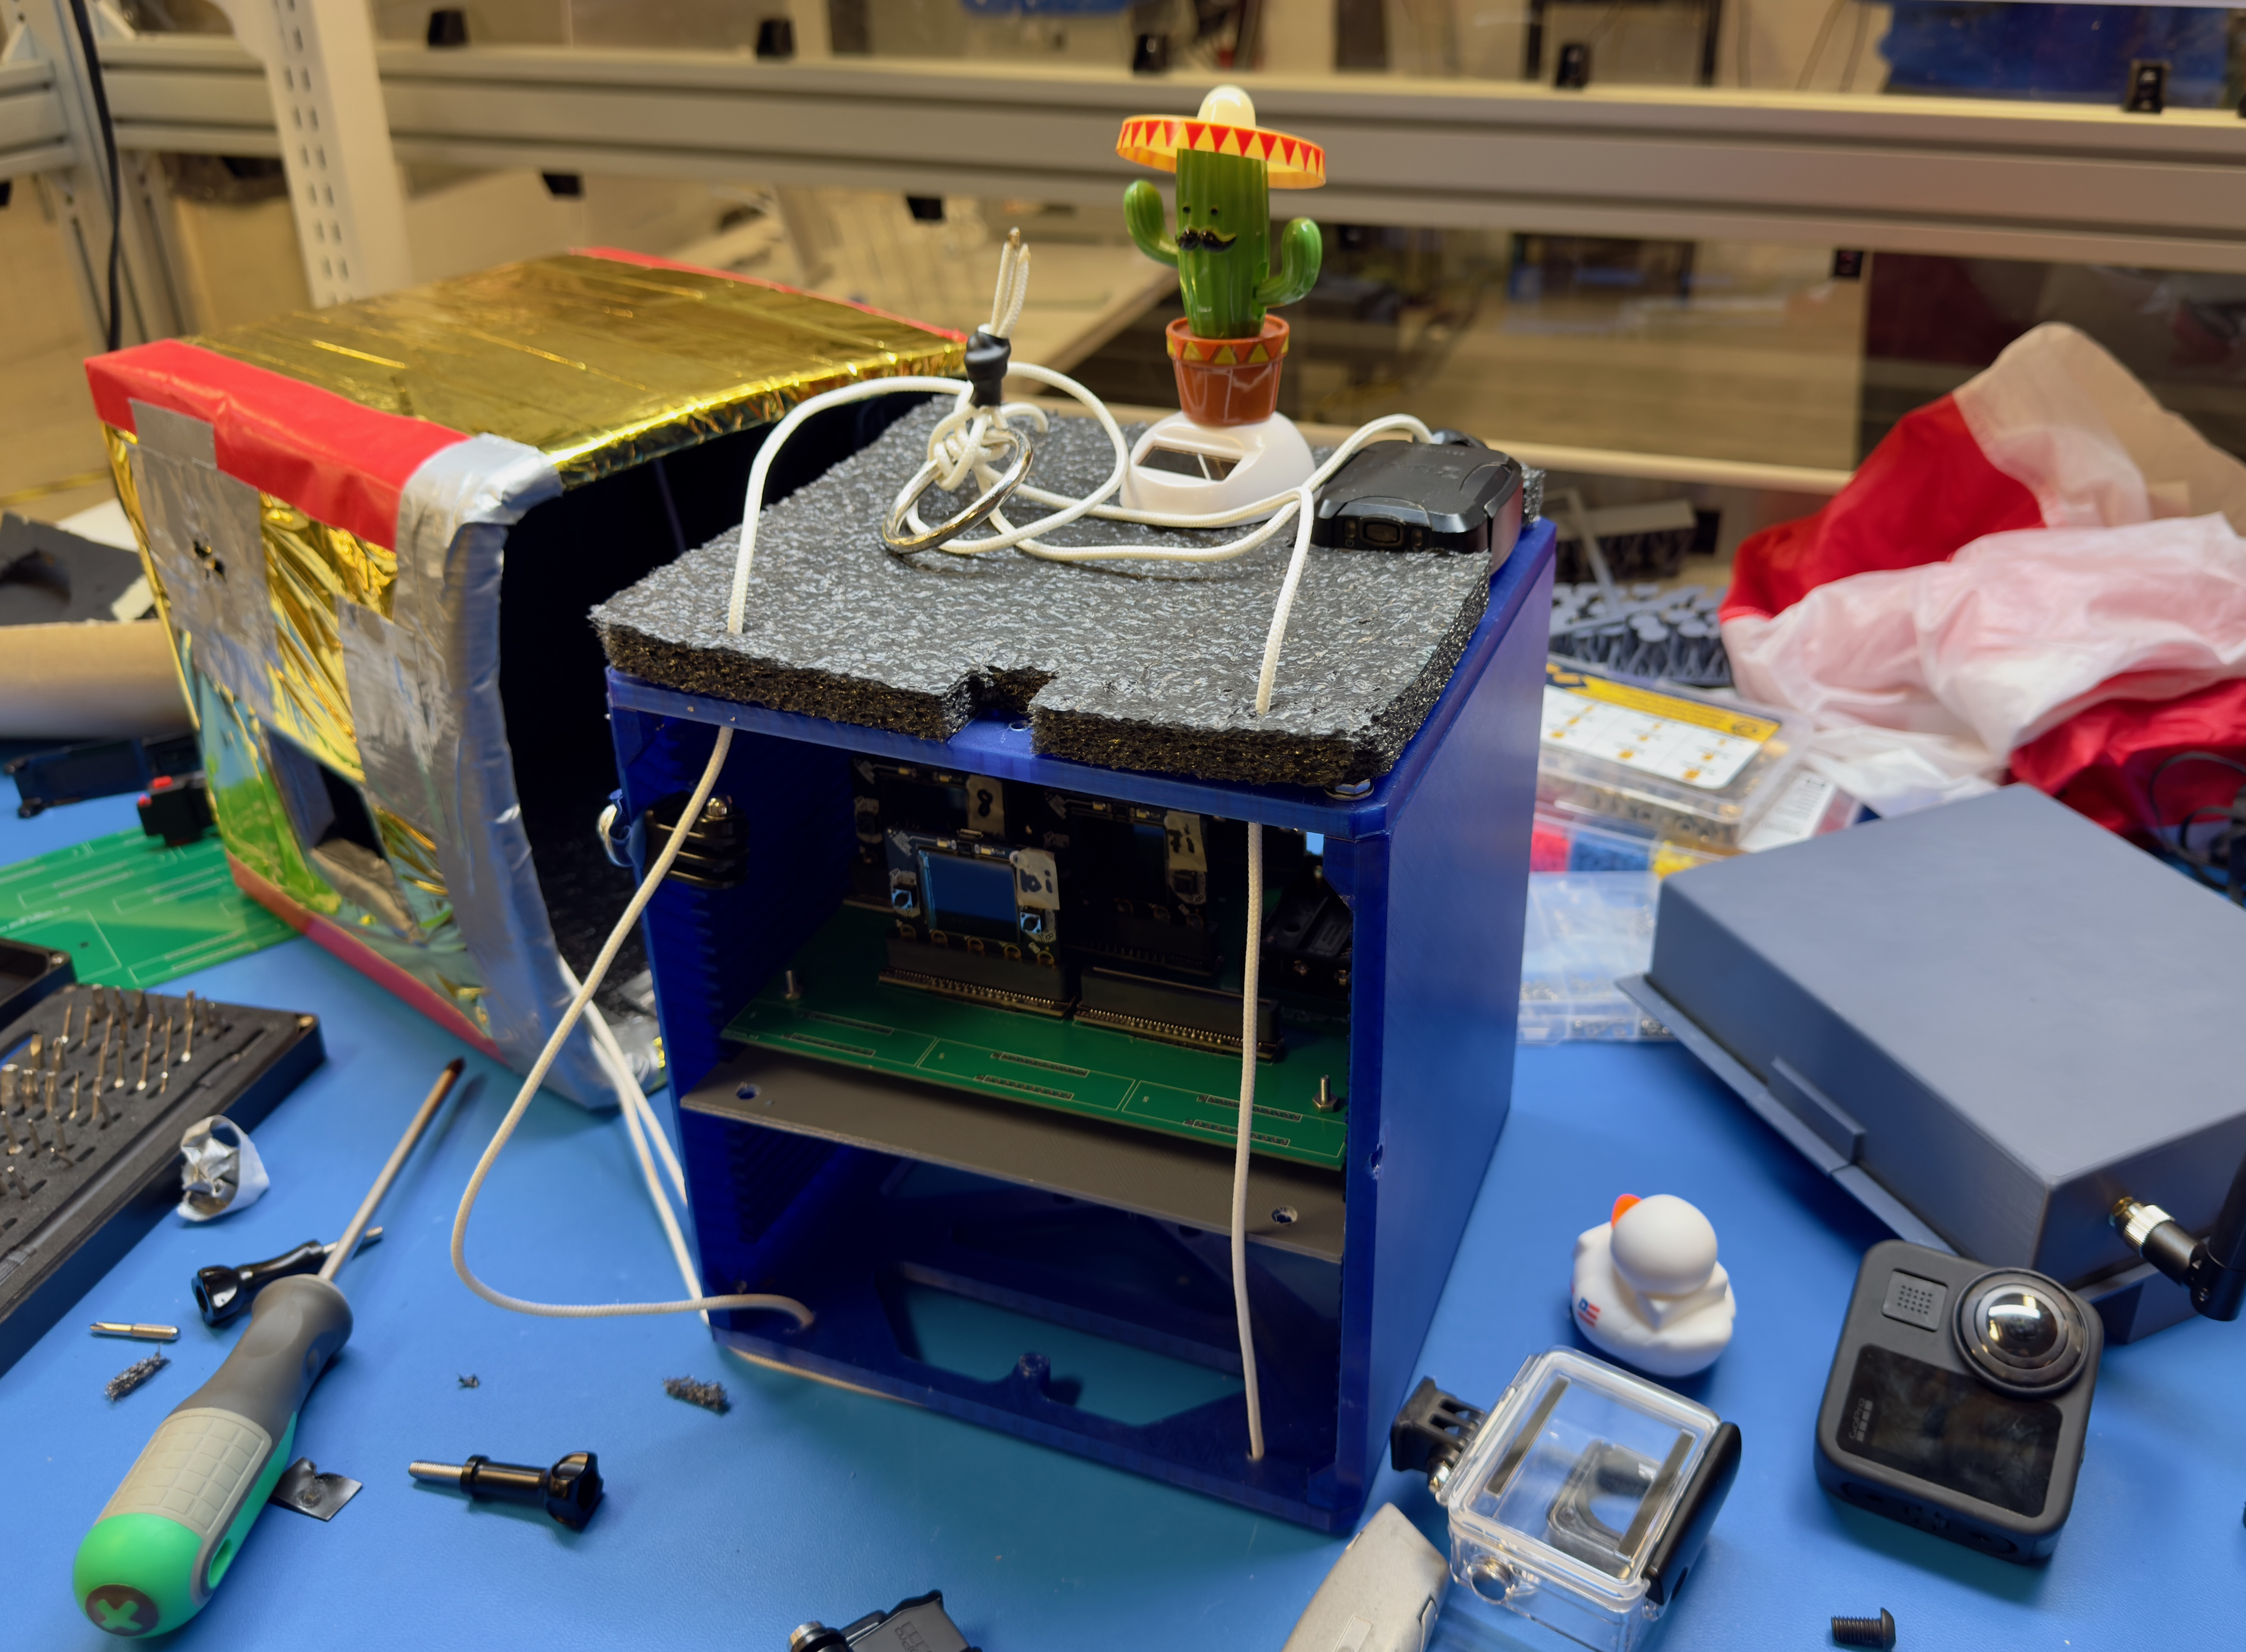
\includegraphics[width=.4\textwidth]{figures/IMG_5594.jpeg}
    \captionsetup{justification=centering}
    \caption{PET-G version of Gemini getting prepped for an upcoming launch}
    \label{fig:gemini}
\end{figure}

The project system comprises a modular drone platform shown in Figure \ref{fig:gemini} designed for package delivery. It includes a GPS-based navigation system, a payload delivery mechanism, and a monitoring dashboard for real-time tracking. These components work together to ensure the system can operate autonomously and deliver packages accurately.

The drone platform is built with scalability and modularity in mind. This design approach allows for future integration of additional features, such as collision avoidance or enhanced battery capacity. Testing and validation will focus on system reliability and performance in various environmental conditions.

This semester, the team focuses on integrating the payload mechanism with the navigation system. By achieving this milestone, the project will be ready for a comprehensive test phase, bringing it closer to meeting its objectives. The final goal is to deliver a functional system prototype that can perform consistently under real-world conditions. 

\textbf{Guiding Questions:}
\begin{itemize}
    \item What are the main components of your project?
    \item How will these components work together?
    \item Why does your project exist?
    \item What problem are you solving, or what opportunity are you addressing?
\end{itemize}

\subsection{Background}
Provide a short background on the project. Summarize previous accomplishments, especially of the prior semester. This should be two to three paragraphs. 

\textbf{Example:} \\
This project builds on work completed during the previous semester. Last semester, the team successfully designed and tested a navigation algorithm that enables the drone to follow predefined routes. This semester focuses on integrating payload handling capabilities and improving the drone's stability during flight.

In addition, the team identified several areas for improvement during initial testing. These include enhancing the drone's performance in windy conditions and optimizing battery life. Addressing these challenges will ensure the system meets its design objectives and delivers consistent results.

This semester, the team is leveraging stakeholder feedback to refine the design. Collaboration with industry partners and competition organizers has provided valuable insights that inform the development process. The team's goal is to demonstrate a fully functional prototype that meets all specified requirements by the end of the semester.


\textbf{Guiding Questions:}
\begin{itemize}
    \item What has been accomplished so far?
    \item What key lessons or insights were gained from previous work?
\end{itemize}

\subsection{Stakeholders, Customers, and End Users}
This section will explain the individuals and organizations that have a stake in or a stake in the project's success. Competition projects should list the organization running the competition as the customer. If you receive funding from an organization, they would be a stakeholder. Service projects should list any current or potential customers they plan to work with. Industry projects should also list that industry as a customer. Make to Innovate is always listed as a stakeholder, as we have a vested interest in you completing your project. Again, we expect around one to three paragraphs.

\textbf{Example:}
The stakeholders for this project include Make to Innovate, and Company XYZ. Make to Innovate, as the program supporting this project has a vested interest in ensuring its success and providing students with valuable learning experiences. Company XYZ, the project's funding partner, is directly interested in the deliverables, as they are exploring similar technologies for their operations.

The end users of the project are logistics companies needing small-package delivery solutions. These companies benefit from a reliable and efficient drone system that reduces delivery time and costs. The insights gained from this project can help end users better understand autonomous delivery's feasibility and practical challenges.

The primary customers are the participants in the ABC Drone Competition. The competition organizers expect a functional and competitive drone system. The system must meet their requirements and showcase innovation in autonomous flight and package delivery. All stakeholders, customers, and end users are listed in Table \ref{tab:stakeholders}.

\begin{table}[ht!]
    \centering
    \begin{tabular}{|l|l|}
        \hline
        \textbf{Category} & \textbf{Description} \\ \hline
        Stakeholders & Make to Innovate, Company XYZ (funding partner) \\ \hline
        End Users & Logistics companies needing small-package delivery solutions \\ \hline
        Customers & Participants in the ABC Drone Competition \\ \hline
    \end{tabular}
    \caption{Example of Stakeholders, Customers, and End Users}
    \label{tab:stakeholders}
\end{table}

\textbf{Guiding Questions:}
\begin{itemize}
    \item Who benefits directly and indirectly from your project?
    \item Are there organizations funding or supporting your project?
\end{itemize}

\newpage
\section{Project Development Plan}

\subsection{Project Objectives and Goals}
Clearly state the objectives and goals of your project for the semester. Write 1–3 paragraphs. Each paragraph must have at least three sentences.

\textbf{Example:}

The primary objective of this project is to design and implement a drone system capable of delivering packages to a specific location with an accuracy of 5 meters. The team aims to develop and integrate an autonomous navigation system with a payload delivery mechanism to achieve this. These objectives align with the project's mission to demonstrate the feasibility of autonomous drone delivery.

Another key objective is to optimize the drone's flight performance. This includes achieving a flight time of at least 15 minutes while carrying a 1 kg payload. The team will also focus on improving stability during flight, particularly in adverse weather conditions.

The project goals include winning the ABC Drone Competition and showcasing the final prototype to stakeholders. By meeting these goals, the team will demonstrate the technical and practical value of the system. Additionally, achieving these goals will provide valuable insights for future project iterations.

\textbf{Guiding Questions:}
\begin{itemize}
    \item What measurable outcomes are you aiming for this semester?
    \item Are these objectives SMART (Specific, Measurable, Achievable, Relevant, Time-bound)?
\end{itemize}

\subsection{Project Scope of Work and Boundaries}
Define the scope of work and boundaries for your project. Write 1–3 paragraphs. Each paragraph must have at least three sentences.

\textbf{Example:}

This project's scope includes designing, building, and testing an autonomous drone platform for package delivery. Key tasks involve integrating the payload mechanism, improving navigation algorithms, and conducting flight tests. All work will focus on achieving the objectives defined for this semester.

Certain activities are explicitly outside the scope of this project. For example, integrating the drone system with third-party logistics software is not part of the current effort. Similarly, the project will not address regulatory approvals or large-scale manufacturing issues.

The team will focus exclusively on tasks that can be completed within the semester timeline. This includes delivering a functional prototype and a comprehensive project report. By clearly defining the scope, the team ensures that resources are allocated efficiently and efforts remain focused on the primary objectives.

\textbf{Guiding Questions:}
\begin{itemize}
    \item What will your team do, and what is explicitly excluded?
    \item How will you define the limits of your work?
\end{itemize}

\subsection{Project Requirements}

Describe the requirements that define the scope and functionality of your project. Write 1–3 paragraphs. Each paragraph must have at least three sentences.

\textbf{Example:}

The project requirements define the technical and functional expectations for the drone system. We have listed our requirements in Table \ref{tab:req} with a functional and non-functional requirements breakdown. The primary requirement is that the drone autonomously navigates to a delivery point within a 5-meter accuracy while carrying a payload of up to 1 kg. Additionally, the system must operate for at least 15 minutes on a single battery charge, ensuring sufficient delivery time within an urban environment.

To ensure reliability, the drone must include obstacle detection and avoidance capabilities. This will minimize the risk of collisions and enhance the system's performance in dynamic environments. Furthermore, the payload delivery mechanism must function seamlessly, releasing the package only when it reaches the designated drop-off point.

Non-functional requirements include maintaining a lightweight design for optimal flight performance and ensuring safety and regulatory standards compliance. The system must also include a user-friendly interface for real-time monitoring and control. These requirements provide a clear framework for the team to guide their design, development, and testing efforts.

\begin{table}[h!]
    \centering
    \begin{tabular}{|l|l|l|}
        \hline
        \textbf{Requirement Type} & \textbf{Description} & \textbf{Priority} \\ \hline
        Functional & Autonomous navigation to delivery point within 5m accuracy & High \\ \hline
        Functional & Payload capacity of 1 kg & High \\ \hline
        Functional & Minimum flight time of 15 minutes & High \\ \hline
        Functional & Obstacle detection and avoidance & Medium \\ \hline
        Non-Functional & Lightweight design for optimal flight performance & Medium \\ \hline
        Non-Functional & Compliance with safety and regulatory standards & High \\ \hline
        Non-Functional & User-friendly interface for real-time monitoring & Low \\ \hline
    \end{tabular}
    \caption{Project Requirements and Priorities}
    \label{tab:req}
\end{table}

\textbf{Guiding Questions:}
\begin{itemize}
    \item What are the functional requirements (what the system must do)?
    \item What are the non-functional requirements (constraints on how the system works)?
    \item Which requirements are the highest priority for project success?
\end{itemize}

\newpage
\section{Project Implementation Plan}
Please provide an overview of how your project will be implemented.

\textbf{Example:}

The implementation plan for this project begins with finalizing the system design and procuring the necessary materials. This will be followed by integrating hardware and software components, ensuring seamless operation. The final phase will involve testing the system in controlled environments to identify and resolve any issues.

As required by Make to Innovate, regular team meetings and progress reviews will help ensure the project stays on track. All team members will present their work at the weekly meeting and additional questions can be asked at these meetings. Additional lab times will be held on Sunday afternoon. These work sessions will allow team members to work together to accomplish their goals. 

The leadership group, consisting of the \pmgfull{} and the \tlfull{}s, will meet once a week on Sunday. In this meeting, all tasks in YouTrack will be reviewed, and new tasks will be generated and assigned. This team's goal is to be at least three weeks ahead in generating tasks. 

\subsection{Project Phases, Milestones, and Major Tasks}
Outline the timeline for your project, including key milestones and deadlines. Write 1–3 paragraphs. Each paragraph must have at least three sentences.

\textbf{Example:}

The project will be executed in a phased approach, with key milestones to track progress. These include completing the hardware assembly by the semester's midpoint and initiating system testing shortly thereafter. Once testing is complete, we will verify the results with the baseline data we collected in the previous semester. A summary of the different phases with an estimated completion date is provided in Table \ref{tab:phases}.

\begin{table}[ht!]
    \centering
    \begin{tabular}{|l|c|c|}
        \hline
        \textbf{Phase} & \textbf{Tasks} & \textbf{Completion Date} \\ \hline
        Phase 1 & Finalize system design and procure materials & February 15, 2025 \\ \hline
        Phase 2 & Assemble and integrate components & March 25, 2025 \\ \hline
        Phase 3 & Testing and final deliverables & April 28, 2025 \\ \hline
    \end{tabular}
    \caption{Project Phase Plan}
    \label{tab:phases}
\end{table}

The project timeline begins with the finalization of the system design during the first four weeks of the semester. This phase includes team brainstorming sessions and mentor feedback to refine the design. Material procurement will be completed concurrently to avoid delays.

The second phase involves hardware assembly and integration, scheduled for weeks 5–9. This phase will also include initial testing to ensure all components function as expected. Weekly progress meetings will be held to address any issues and stay on track.

The final phase focuses on testing, documentation, and preparing the demonstration. This phase, scheduled for weeks 10–15, will include rigorous system testing under real-world conditions. Following this timeline, the team aims to deliver all project deliverables on schedule. 

Finally, the team will document the results and prepare for the final demonstration at the M2I Expo. This phase will include creating a comprehensive report and a video presentation. A list of the major tasks and milestones, along with estimated time and completion dates, are shown in Table \ref{tab:majortasks}. By adhering to this plan, the team aims to meet all deliverables by the end of the semester.

\begin{table}[ht!]
    \centering
    \begin{tabular}{|l|c|c|}
        \hline
        \textbf{Task} & \textbf{Estimated Time (Hours)} & \textbf{Completion Date} \\ \hline
        Finalize system design & 20 & February 15, 2025 \\ \hline
        Procure materials & 10 & February 20, 2025 \\ \hline
        Assemble hardware components & 40 & March 10, 2025 \\ \hline
        Integrate hardware and software & 50 & March 25, 2025 \\ \hline
        Conduct system testing & 30 & April 10, 2025 \\ \hline
        Prepare final documentation & 25 & April 25, 2025 \\ \hline
    \end{tabular}
    \caption{Major Tasks and Timelines for Project Implementation}
    \label{tab:majortasks}
\end{table}

\textbf{Guiding Questions:}
\begin{itemize}
    \item What are the major phases of your project?
    \item When do you expect each phase to be completed?
    \item What are the major tasks required to complete your project?
    \item How much time is estimated for each task?
    \item What are the deadlines for completing these tasks, phases, and milestones?
\end{itemize}

\subsection{Project Deliverables}
Describe the tangible items your team will produce during the semester. There should be a correlation between your deliverables and the milestones defined above. Write 1–3 paragraphs. Each paragraph must have at least three sentences.

\textbf{Example:}

The primary deliverable for this project is a functional drone prototype capable of autonomous navigation and package delivery. The prototype will include integrated hardware and software systems allowing accurate navigation and reliable payload handling. This deliverable will be the foundation for testing and demonstrating the project's feasibility.

Another key deliverable is the final project report, which will document the system design, testing procedures, and results. The report will include detailed analyses of system performance, challenges encountered, and recommendations for future work. This document will be presented to stakeholders as evidence of the project's progress and success.

Additionally, the team will prepare a demonstration video showcasing the drone's capabilities in action. This video will highlight the system's functionality and provide visual proof of its performance. These deliverables demonstrate the team's achievements and lay the groundwork for future project iterations. All deliverables, including the estimated amount of time and completion dates, are shown in Table \ref{tab:deliverables}.

\begin{table}[ht!]
    \centering
    \begin{tabular}{|l|c|c|}
        \hline
        \textbf{Deliverable} & \textbf{Estimated Time (Hours)} & \textbf{Completion Date} \\ \hline
        Functional drone prototype & 120 & April 15, 2025 \\ \hline
        Final project report & 30 & April 25, 2025 \\ \hline
        Demonstration video & 15 & April 28, 2025 \\ \hline
    \end{tabular}
    \caption{Project Deliverables, Estimated Time, and Completion Dates}
    \label{tab:deliverables}
\end{table}

\textbf{Guiding Questions:}
\begin{itemize}
    \item What tangible items will your team produce?
    \item How will these items demonstrate project success?
    \item How much time is required to complete each deliverable?
    \item What are the expected completion dates for your deliverables?
\end{itemize}

\subsection{Resource Management Plan}
Outline the resources your team needs to complete the project, including materials, facilities/equipment, funding, and personnel. This section should have a table with a rough outline of costs (materials, equipment, travel, etc). It should also include what funding you have secured so far (ISGC funds, for example). The table in the example shows the key personnel. Eventually, this section will have a full organization chart and student list once assigned. 

\textbf{Example:}

This project requires several key resources to ensure its success. The materials include electronic components such as GPS modules, sensors, and batteries for the drone. The drone uses these devices for autonomous flight. The team also needs access to the university's wind tunnel lab for aerodynamic testing and a budget of \$2,000 for material procurement and \$5,000 for travel costs. The travel will be to the Drone Competition in Fergus Falls, Minnesota, on April 28th, 2025. The team has already secured a \$5,000 Student Hands-On (SHO) grant from the Iowa Space Grant Consortium. We are therefore asking for \$2,000 from Make to Innovate to complete our project. 

Personnel resources include team members with programming, hardware assembly, and testing expertise. Collaboration with external mentors and advisors will also be essential for addressing technical challenges. The team will assign roles to ensure the efficient allocation of these human resources. Table \ref{tab:orgchart} lists key personnel for our project.

\begin{table}[ht!]
    \centering
    \begin{tabular}{|l|l|l|}
        \hline
        \textbf{Role} & \textbf{Responsibility} & \textbf{Assigned Member} \\ \hline
        Project Manager & Oversees overall project activities & John Smith \\ \hline
        Hardware Team Leader & Leads design and assembly of hardware components & Jane Doe \\ \hline
        Software Team Leader & Oversees software development and integration & Emily Davis \\ \hline
        Testing Team Leader & Manages testing and validation processes & Michael Lee \\ \hline
        Safety Officer & Ensures safety compliance in all project activities & Sarah Johnson \\ \hline
        Travel Coordinator & Plans and coordinates travel logistics & David Wilson \\ \hline
    \end{tabular}
    \caption{Organizational Roles and Responsibilities}
    \label{tab:orgchart}
\end{table}

Additionally, software tools such as SolidWorks for design and MATLAB for simulation will be required. As Iowa State University provides these, no additional licenses are needed, ensuring their availability throughout the semester. The project aims to stay on schedule and within budget by managing these resources effectively. A listing of resources needed is shown in Table \ref{tab:resources}.

\begin{table}[ht!]
    \centering
    \begin{tabular}{|l|l|c|}
        \hline
        \textbf{Resource Type} & \textbf{Description} & \textbf{Estimated Cost (\$)} \\ \hline
        Materials & GPS modules, sensors, batteries & \$2,000 \\ \hline
        Facilities & Access to wind tunnel lab & No Cost \\ \hline
        Software & SolidWorks, MATLAB, and testing tools & No Cost \\ \hline
        Travel & Travel to the competition & \$5,000 \\ \hline
        Budget & General project budget & \$7,000 \\ \hline
        Funding Secured & Make to Innovate allocation & -\$2,000 \\ \hline
        Funding Secured & ISGC & -\$5,000 \\ \hline
    \end{tabular}
    \caption{Resources Required for the Project}
    \label{tab:resources}
\end{table}

\textbf{Guiding Questions:}
\begin{itemize}
    \item What materials and equipment are required for your project?
    \item What facilities will you need access to?
    \item What is your estimated budget for resources?
    \item Why do you need these resources?
    \item Have you secured any additional funding?
\end{itemize}

\subsection{Project Operational Plan}
Describe how your team will operate to ensure successful project completion. Write 1–3 paragraphs. Each paragraph must have at least three sentences.

\textbf{Example:}

The team will hold weekly meetings to review progress, assign tasks, and address challenges. These meetings will include a review of the project timeline and any necessary adjustments. Subteams focusing on hardware, software, and documentation will report updates during each meeting.

The operational structure includes assigning a team leader to oversee the project's progress. Each subteam will have a designated lead responsible for specific deliverables. The team will use Microsoft Teams for communicating and storing documents and design files. The software developed will be kept in a GitHub repository. Regular updates will be shared with mentors and stakeholders to gather feedback. By adhering to this operational plan, the team ensures that all members stay informed and focused on project goals.

\textbf{Guiding Questions:}
\begin{itemize}
    \item How will your team communicate and collaborate?
    \item What roles and responsibilities are assigned to team members?
    \item What tools will you use for task tracking and documentation?
\end{itemize}

\subsection{Project Risks and Contingency Plan}
Identify potential risks to the project and describe contingency plans for each risk. Write 1–3 paragraphs. Each paragraph must have at least three sentences.

\textbf{Example:}

One of the main risks to this project is hardware failure during testing. This risk could result in delays if replacement parts are not readily available. To mitigate this, the team has budgeted for spare components and plans to perform thorough pre-flight checks.

Another potential risk is software bugs affecting the drone's navigation system. These issues could lead to unexpected behavior or crashes. The team will address this risk by conducting incremental testing and debugging after each development milestone.

A third risk is project delays due to unforeseen circumstances, such as team member absences or supply chain issues. The team has developed a contingency plan that includes cross-training members and ordering materials early. These measures ensure the project stays on track despite potential disruptions.

\begin{table}[ht!]
    \centering
    \begin{tabular}{|l|l|l|}
        \hline
        \textbf{Risk} & \textbf{Impact} & \textbf{Contingency Plan} \\ \hline
        Hardware failure & Delays due to repair or replacement & Budget for spare parts; pre-flight checks \\ \hline
        Software bugs & Navigation issues or crashes & Incremental testing and debugging \\ \hline
        Delays (e.g., absences) & Missed deadlines & Cross-train team members; order materials early \\ \hline
    \end{tabular}
    \caption{Project Risks and Contingency Plans}
\end{table}

\textbf{Guiding Questions:}
\begin{itemize}
    \item What risks could hinder your project's success?
    \item How significant is the impact of each risk?
    \item What contingency plans are in place to address these risks?
\end{itemize}

\section{Conclusion}
Write any concluded thoughts or summarize your document.
% -----------------------------------------
\newpage

% begin sign off -- {{{
\subsection{Sign-Off}
\textit{To be completed by all students after reading and agreeing to the plan outlined in this document. The complete list of students will be included after final assignments have been made. The faculty advisor will initialize the boxes to confirm.}
\vspace{.02cm}
\ \\

\textbf{Title} \tabto{20em}\textbf{Signature}\hspace{10em}\textbf{Date}
\begin{checklist}
    \item \pmgfull \tabto{20em}\rule{10em}{0.4pt}\hspace{5em}\rule{10em}{0.4pt}
    \item \tlfull  \tabto{20em}\rule{10em}{0.4pt}\hspace{5em}\rule{10em}{0.4pt}
    \item \tmfull  \tabto{20em}\rule{10em}{0.4pt}\hspace{5em}\rule{10em}{0.4pt}
    \item \sofull  \tabto{20em}\rule{10em}{0.4pt}\hspace{5em}\rule{10em}{0.4pt}
    \item \tcfull  \tabto{20em}\rule{10em}{0.4pt}\hspace{5em}\rule{10em}{0.4pt}
\end{checklist}
\setcounter{checklistnum}{0}

% ------------------------------------------
% BIBLIOGRAPHY
% ------------------------------------------
\newpage
\bibliography{references}

% ------------------------------------------
% APPENDICES & ATTACHMENTS
% ------------------------------------------
\newpage
\section{Appendix}
The following section presents supporting documentation for the conclusions presented in the body of this report.

\renewcommand{\thesubsection}{\Alph{subsection}}

\subsection{Gemini Technical Drawings}
\label{appendix:GeminiDrawing}

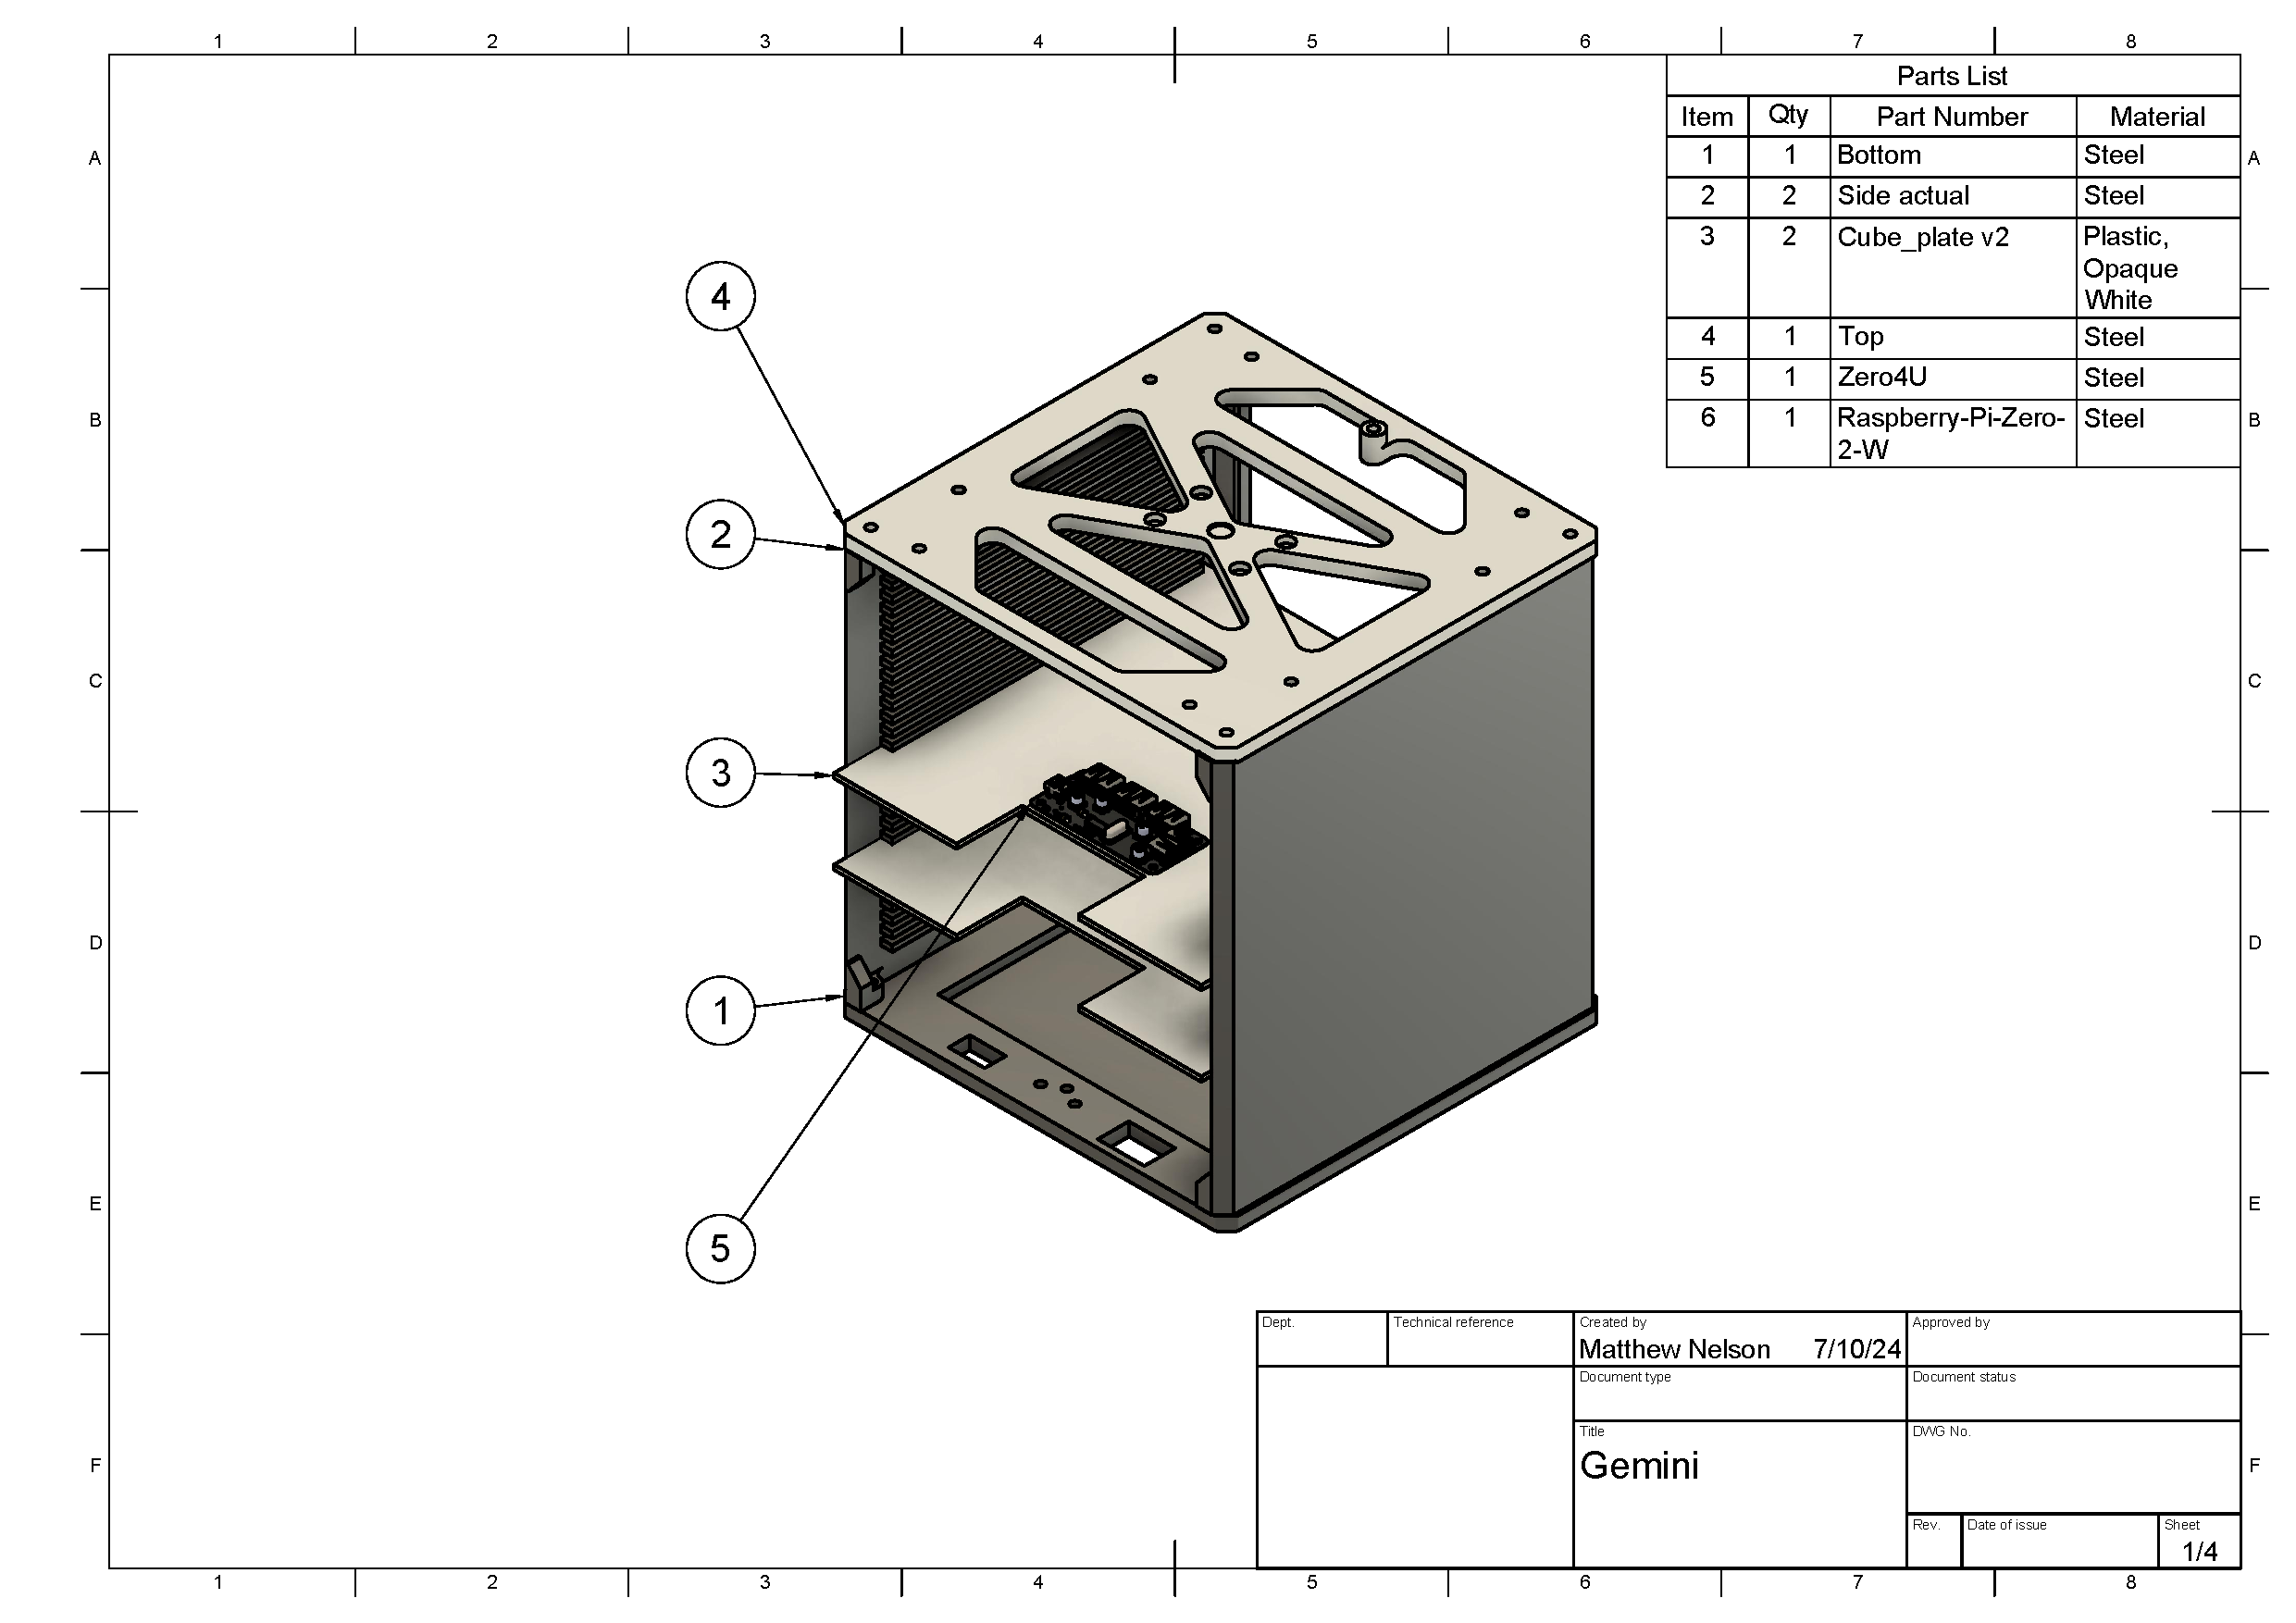
\includepdf[pages=-]{appendix/Gemini Drawing v2.pdf}

\subsection{Kaymont Spec Sheets}
\label{appendix:Kaymont}

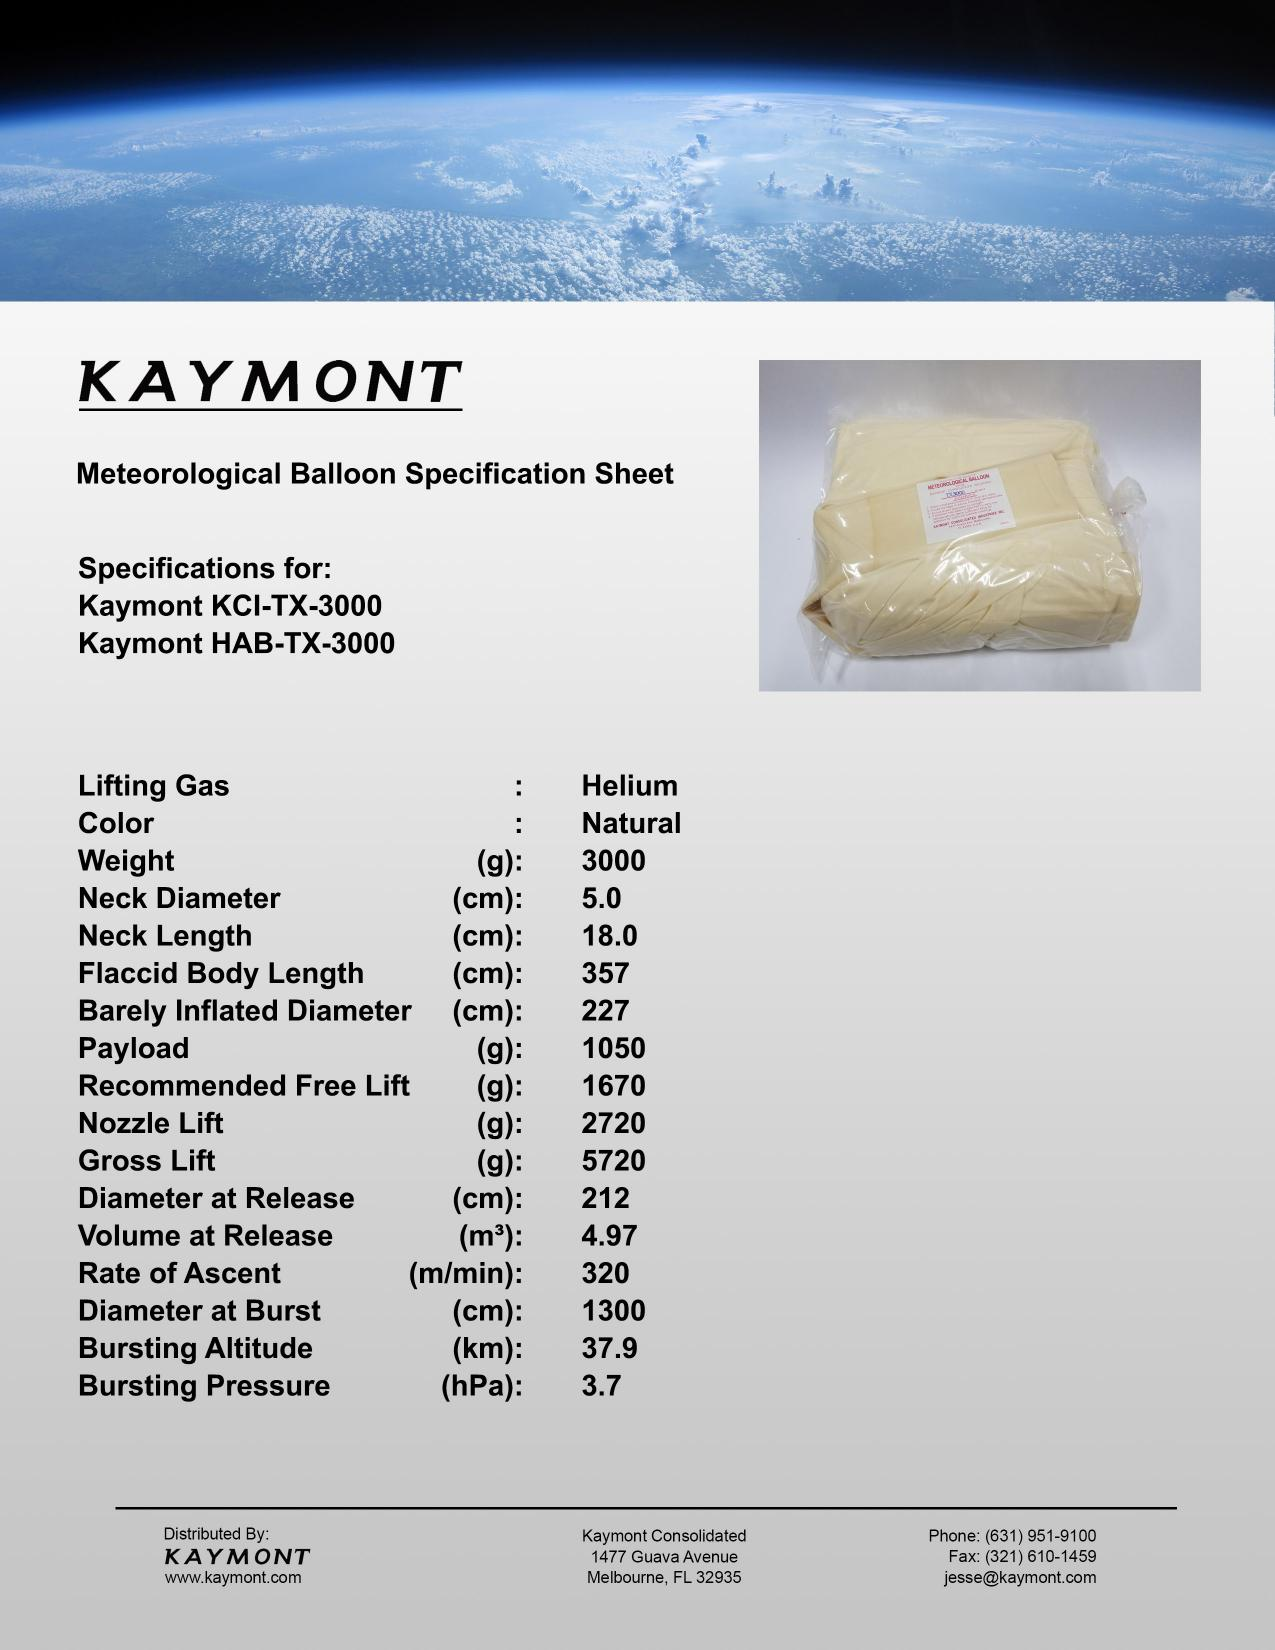
\includepdf[pages=-]{appendix/Kaymont Meteorological Balloon Spec Sheet KCI-TX-3000 PDF-min.pdf}

\end{document}